% !TEX root=report.tex
\section{Features} \label{sec:features}

The featurization function $\Phi(s,h,r)$ maps properties of a couch request $r$ from surfer $s$ to host $h$ to a real-dimensional $D$-vector.
The properties we care about include structured personal information such as age, gender, languages spoken, countries lived in, countries traveled to, and so on.
Additionally, we would like to use user interests, extracted from free form text on their profiles, and their status and activity on the website, e.g. the number of references, number of friends, or message response rate.

We developed a general approach for dealing with a wide variety of features.
For each feature, we construct a histogram whose boundaries are determined by the inverse distribution of values in the training set.
Using this mapping from value to bin we vectorize each feature by mapping it to a binary vector (e.g. $age=27$ to $b=[0,0,0,1,0,\dots]^T$).
Since our feature $\Phi(s,h)$ is based on both the surfer $s$ and the host $h$, the final feature includes this binary vector for each of them, as well as the outer product between the two, $b_s b_h^T$.

The reason for the outer product feature is to capture potential preference combinations.
For example, we are able to model that hosts between $21$ and $25$ years old prefer surfers of the same age, while hosts over $60$ don't have a particular preferences in this regard (as an example).
Other example inlude capturing affinities between genders, countries, spoken languages, certain interest groups, etc.

In addition to these cross-product preference features, we include additional unary features, such as the number of languages in common, and features relating to reputation.
The final feature vector is quite sparse.

\subsection{User interests} \label{subsec:user_interests}

As mentioned, we extract ``interestst'' features from free-form user profile text as additional signal to the feature vector.

\todo{add some more information about interest extraction + interest graph + clustering + interest feature here}
Interest graph: the compatibility strength between surfer and host is determined by $num_overlapping_interest(host, surfer)$ through some type of decaying activation propagation.  This will be based on the "Taste Fabric" paper and the "Semantic Recommendation" paper.  This method assumes homophily and that interests are the strongest attractors between people (doesn't take into account demographics etc.).  This method is reversible.

\begin{figure}[ht]
\centering
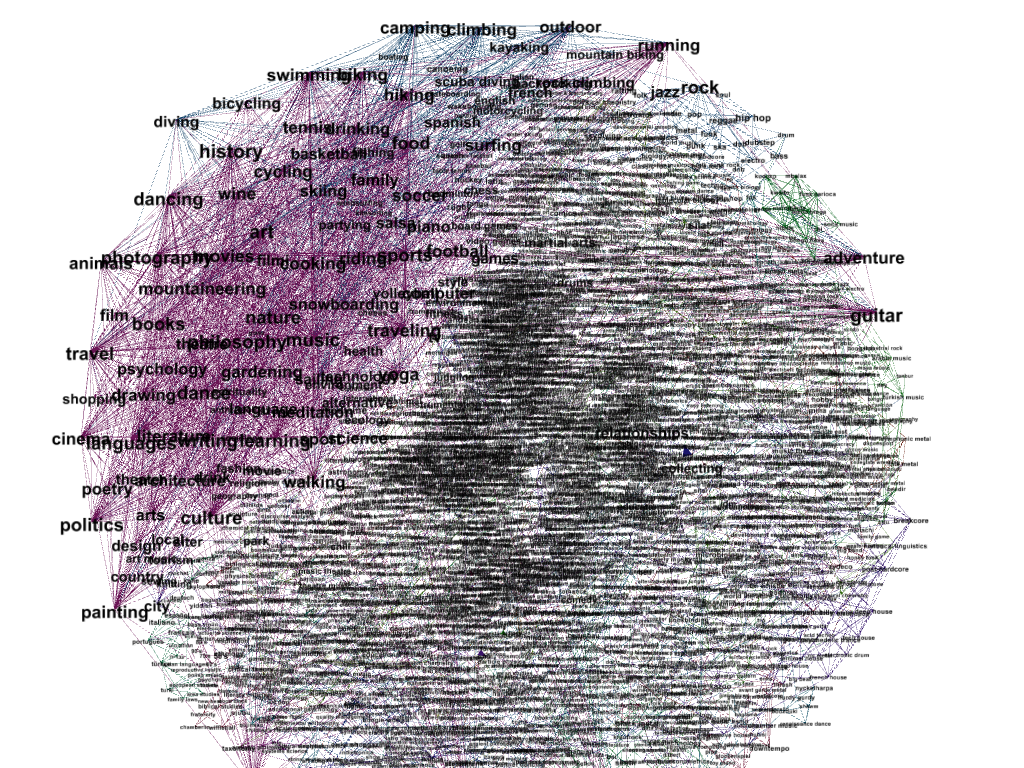
\includegraphics[width=1\linewidth]{figures/interest_graph.png}
\caption{Interest graph.}
\label{fig:interest_graph}
\end{figure}
